\section{Computational experiment}
\subsection{Settings}

This section focuses on the choice of neural network architecture. 
To conduct the experiments, a handwritten digit classification task based on the MNIST dataset \cite{Deng2012} was considered.

To solve this task, we implemented an algorithm for generating a graph neural network architecture. 
The procedure follows an approach similar to neural architecture search \cite{Zoph2017}. 
Let \texttt{MLPblock} denote a node consisting of a linear layer followed by the ReLU activation function. 
Formally,
\begin{equation}
\texttt{MLPblock}(\mathbf{x}) = \textbf{ReLU}(\textbf{Linear}(\mathbf{x})).
\end{equation}

Define \texttt{node\_list} as the list of constructed nodes. 
Initially, \texttt{node\_list} contains two nodes: the input node and a node that maps the input to a latent representation. 
Then, \texttt{n\_iterations} iterations of the algorithm are performed. 
Each iteration consists of four steps.

\begin{description}
\item[\textbf{Step 1.}]
Independently select two parent nodes from \texttt{node\_list}.

\item[\textbf{Step 2.}]
Apply a \texttt{MLPblock} to the first parent node selected in Step~1 and append the resulting node to \texttt{node\_list}.

\item[\textbf{Step 3.}]
Apply a \texttt{MLPblock} to the second parent node selected in Step~1 and append the resulting node to \texttt{node\_list}.

\item[\textbf{Step 4.}]
Apply a \texttt{MLPblock} to combine the outputs obtained in Steps~2 and~3, thereby creating a new node, and append it to \texttt{node\_list}.
\end{description}

After completing all iterations, the algorithm aggregates all terminal (hanging) nodes and applies a final classifier for the MNIST task.

Depending on the value of \texttt{n\_iterations}, the resulting architecture contains a different number of edges (see Figs.~\ref{graph_example_1},~\ref{graph_example_2}).

\begin{figure}[H]
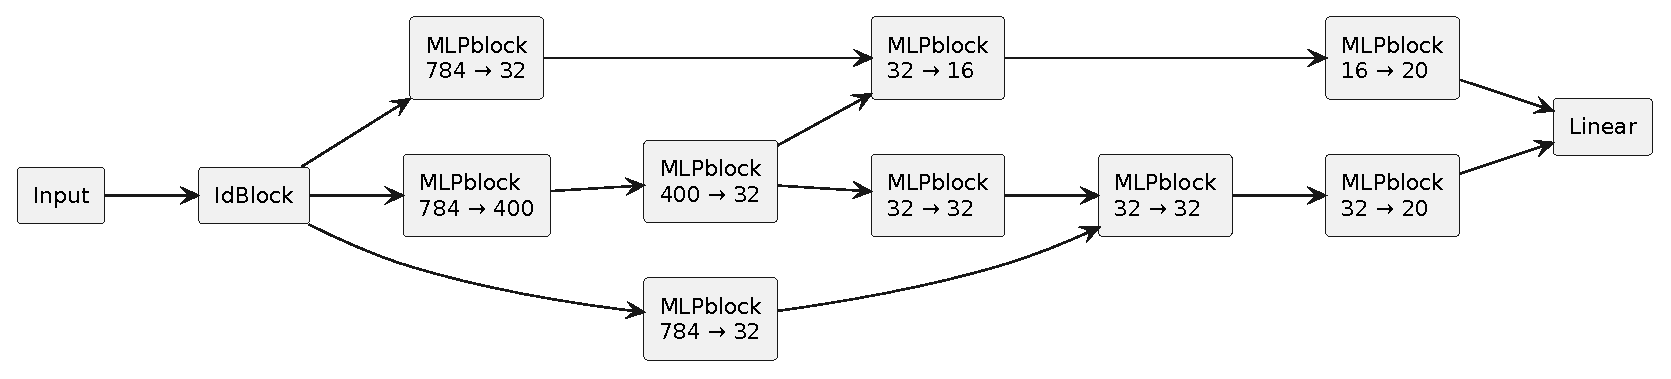
\includegraphics[width=\textwidth]{figs/graph_example_1.eps}
\caption{The generated graph with 14 edges.}
\label{graph_example_1}
\end{figure}

\begin{figure}[H]
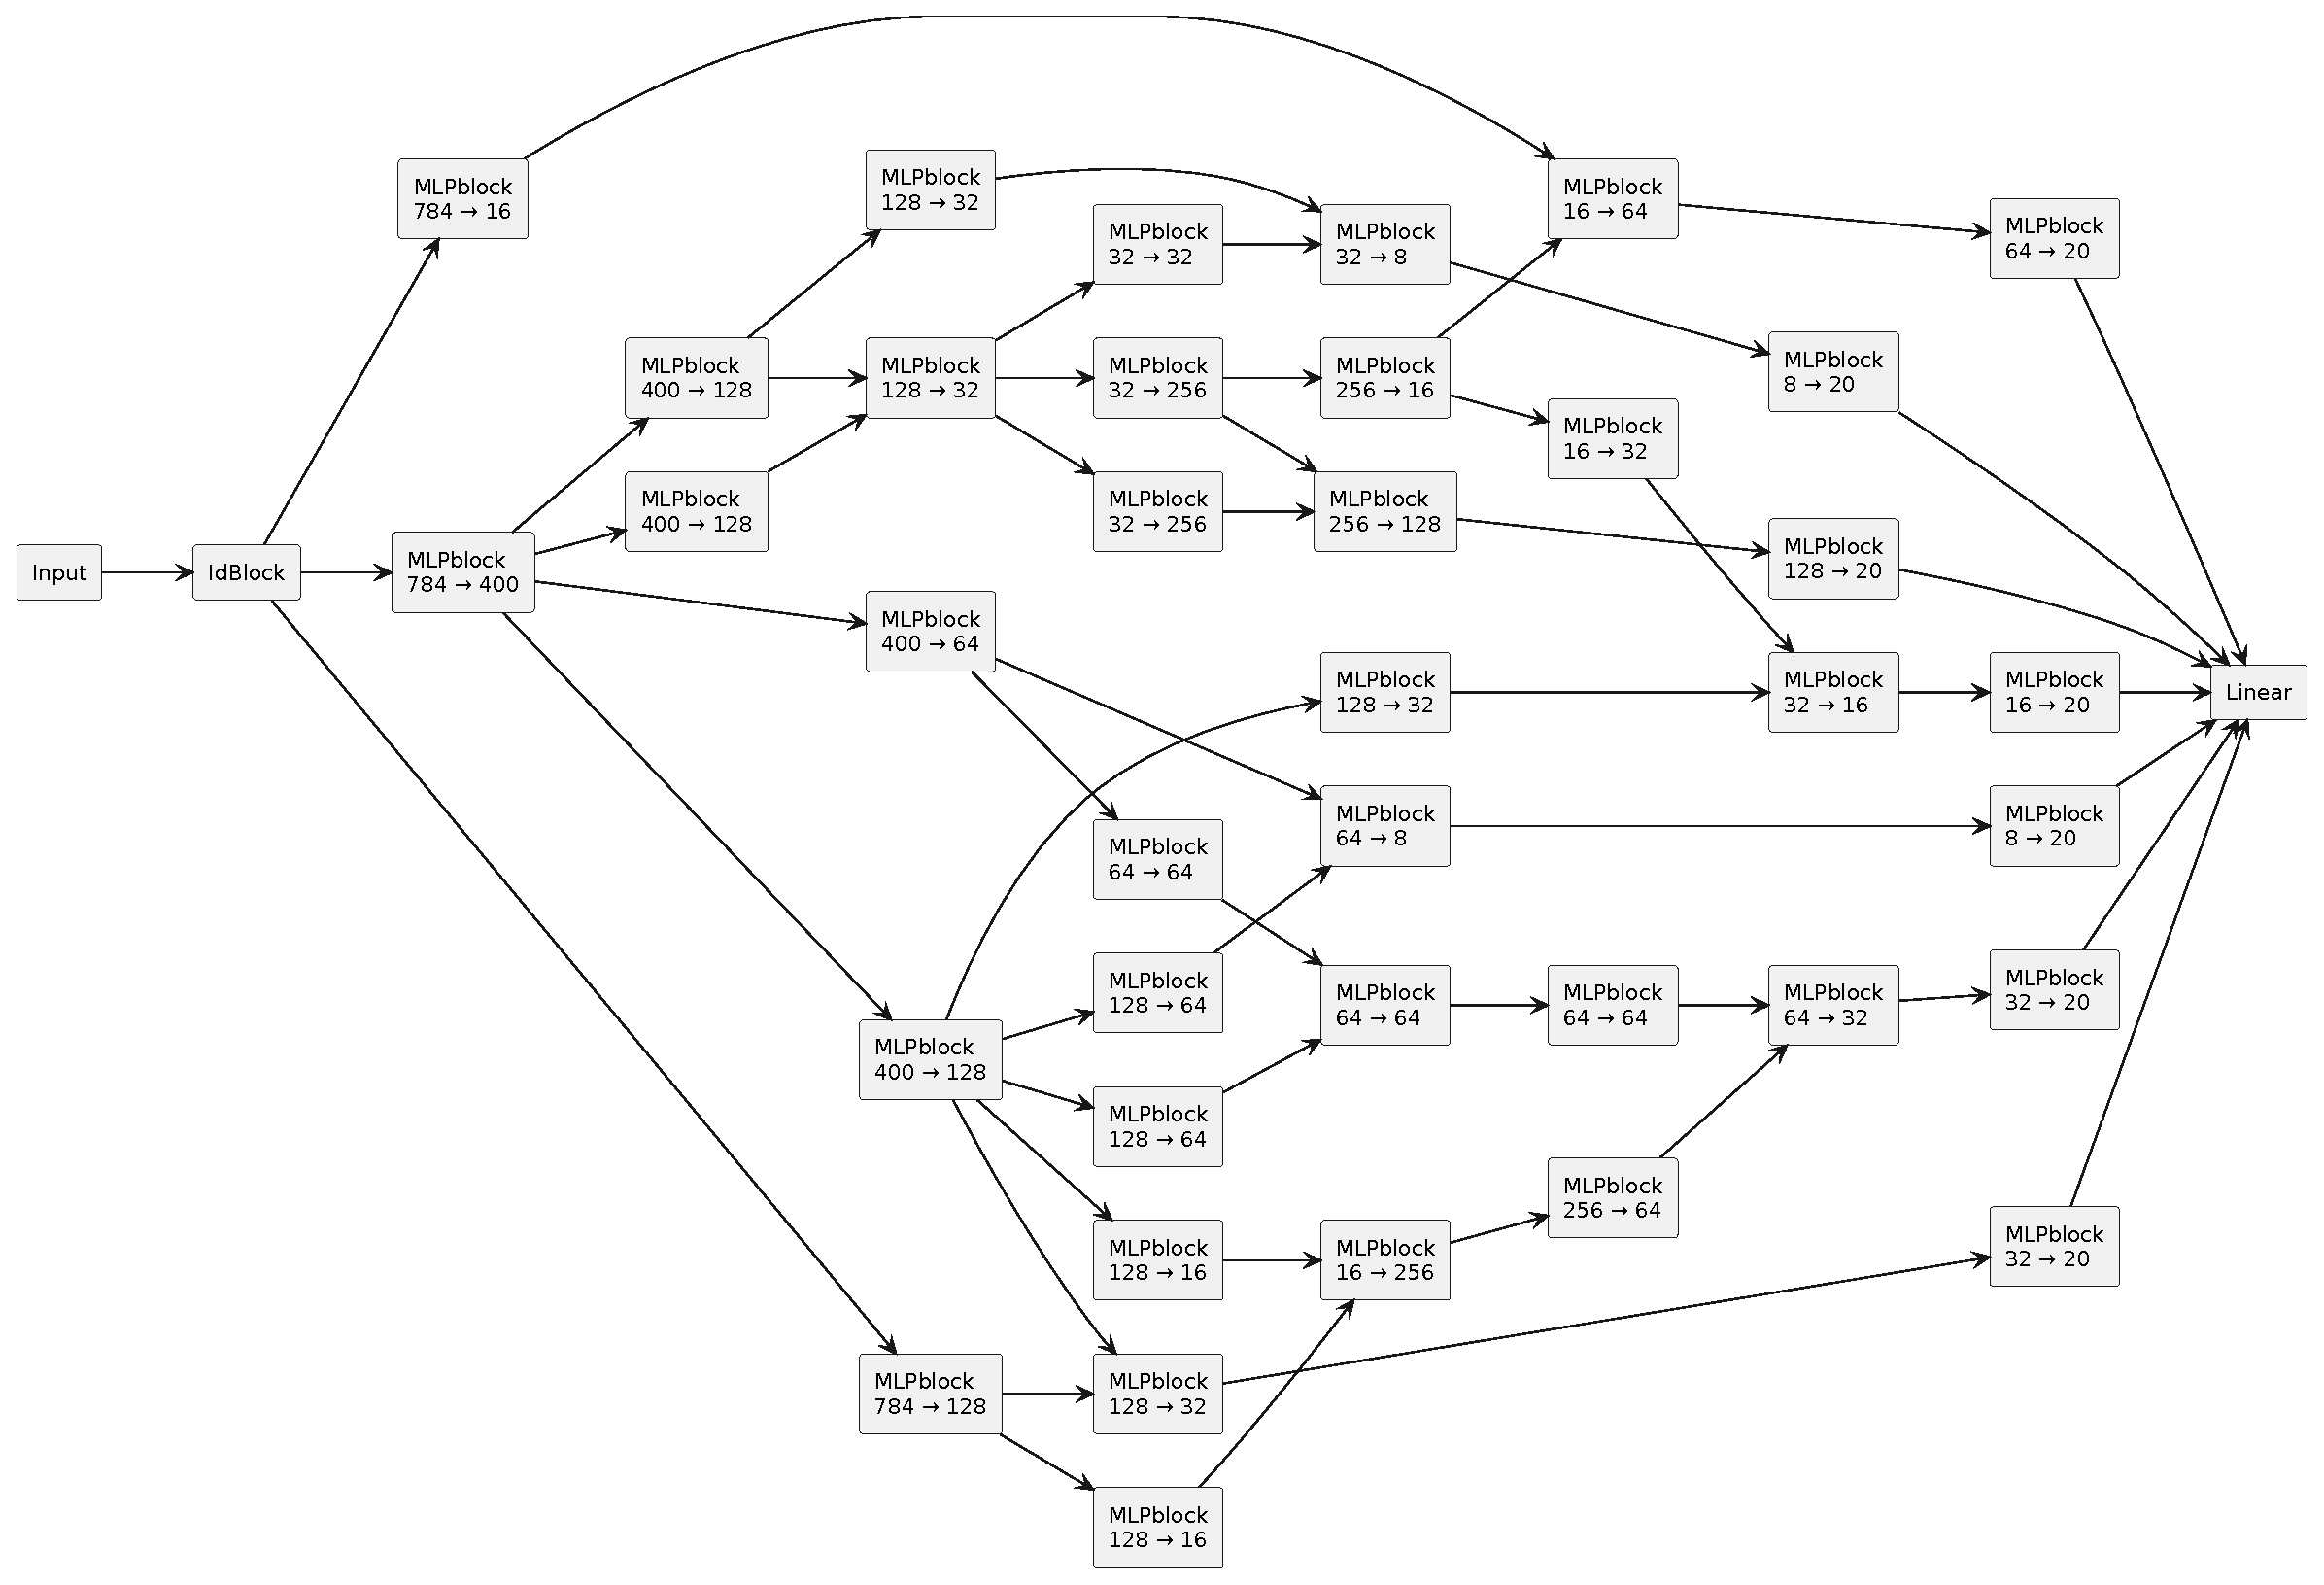
\includegraphics[width=\textwidth]{figs/graph_example_2.eps}
\caption{The generated graph with 56 edges.}
\label{graph_example_2}
\end{figure}

The training set for the surrogate models consists of binary masks containing either all ones, all zeros, or exactly one zero with all remaining entries equal to one. 
Thus, the size of the training set is equal to $(\text{number of edges} + 1)$, which enables a few-shot setting. 
The test set consists of $500$ masks sampled uniformly without replacement.

The following models were compared in the experiments:

\begin{itemize}
\item \textbf{Graph}:
The proposed surrogate graph model.

\item \textbf{FCN}:
A fully connected network with the following architecture:\\
\texttt{Linear(number\_of\_edges, 10), ReLU(), Linear(10, 1)}.

\item\textbf{Linear}:
Linear regression.

\item\textbf{L1}:
Magnitude pruning \cite{Han2015}.

\item\textbf{Taylor expansion}:
The method using the first and second-order Taylor expansions \cite{Molchanov2019}.
\end{itemize}

The \textbf{surrogate graph model} is trained for $3000$ epochs, while the \textbf{FCN model} is trained for $1000$ epochs. 
Both models are optimized using the mean squared error (MSE) loss and the Adam optimizer with learning rate $10^{-3}$.

In the experiments, Spearman and Kendall correlation coefficients between the true and predicted error values were used as evaluation metrics. 
These statistics assess the rank dependence between samples. 
For a more robust evaluation, each experiment was repeated ten times, and the results were averaged.

\subsection{Experiment results}

As shown in Tables~\ref{results_spearman} and~\ref{results_kendall}, the proposed method demonstrates strong performance in the few-shot setting. 
It significantly outperforms the baseline models and provides informative estimates of edge importance.

\begin{table}[H]
\caption{Average Spearman correlation coefficient over 10 runs.}
\label{results_spearman}
\centering
\begin{tabular}{|r|c|c|c|c|}
\hline
\bfseries Model & 10--15 edges & 20--40 edges & 50--100 edges & > 100 edges \\
\hline
Graph  & 0.299 $\pm$ 0.235 & 0.296 $\pm$ 0.178 & 0.349 $\pm$ 0.128 & \textbf{0.411} $\pm$ 0.057 \\
FCN & $-0.009$ $\pm$ 0.213 & $-0.060$ $\pm$ 0.187 & $-0.028$ $\pm$ 0.090 & $-0.053$ $\pm$ 0.099 \\
Linear & 0.060 $\pm$ 0.187 & 0.201 $\pm$ 0.122 & 0.248 $\pm$ 0.090 & 0.294 $\pm$ 0.047 \\
L1 & \textbf{0.547} $\pm$ 0.063 & \textbf{0.505} $\pm$ 0.063 & \textbf{0.369} $\pm$ 0.060 & 0.280 $\pm$ 0.081 \\
Taylor exp.& 0.119 $\pm$ 0.247 & $-0.052$ $\pm$ 0.082 & $-0.136$ $\pm$ 0.076 & $-0.204$ $\pm$ 0.044 \\
\hline
\end{tabular}
\end{table}

\begin{table}[H]
\caption{Average Kendall correlation coefficient over 10 runs.}
\label{results_kendall}
\centering
\begin{tabular}{|r|c|c|c|c|}
\hline
\bfseries Model & 10--15 edges & 20--40 edges & 50--100 edges & > 100 edges \\
\hline
Graph  & 0.253 $\pm$ 0.202 & 0.242 $\pm$ 0.146 & \textbf{0.282} $\pm$ 0.105 & \textbf{0.329} $\pm$ 0.045 \\
FCN & $-0.011$ $\pm$ 0.151 & $-0.042$ $\pm$ 0.128 & $-0.020$ $\pm$ 0.061 & $-0.036$ $\pm$ 0.066 \\
Linear & 0.039 $\pm$ 0.135 & 0.137 $\pm$ 0.083 & 0.167 $\pm$ 0.061 & 0.199 $\pm$ 0.032 \\
L1 & \textbf{0.401} $\pm$ 0.057 & \textbf{0.353} $\pm$ 0.049 & 0.259 $\pm$ 0.041 & 0.192 $\pm$ 0.057 \\
Taylor exp. & 0.094 $\pm$ 0.182 & $-0.033$ $\pm$ 0.055 & $-0.090$ $\pm$ 0.051 & $-0.136$ $\pm$ 0.030 \\
\hline
\end{tabular}
\end{table}

\begin{figure}[H]

\includegraphics[width=\textwidth]{figs/graph_1_iter_2_experiment_6.eps}
\centering

\includegraphics[width=0.7\textwidth]{figs/graph_2_iter_2_experiment_6.eps}
\caption{Scatter plot of true and predicted error values for the baseline comparison. The parameter \texttt{n\_iterations} is set to 2.}
\label{graph_iter_2}
\end{figure}

\begin{figure}[H]

\includegraphics[width=\textwidth]{figs/graph_1_iter_5_experiment_6.eps}
\centering

\includegraphics[width=0.7\textwidth]{figs/graph_2_iter_5_experiment_6.eps}
\caption{Scatter plot of true and predicted error values for the baseline comparison. The parameter \texttt{n\_iterations} is set to 5.}
\label{graph_iter_5}
\end{figure}

\begin{figure}[H]
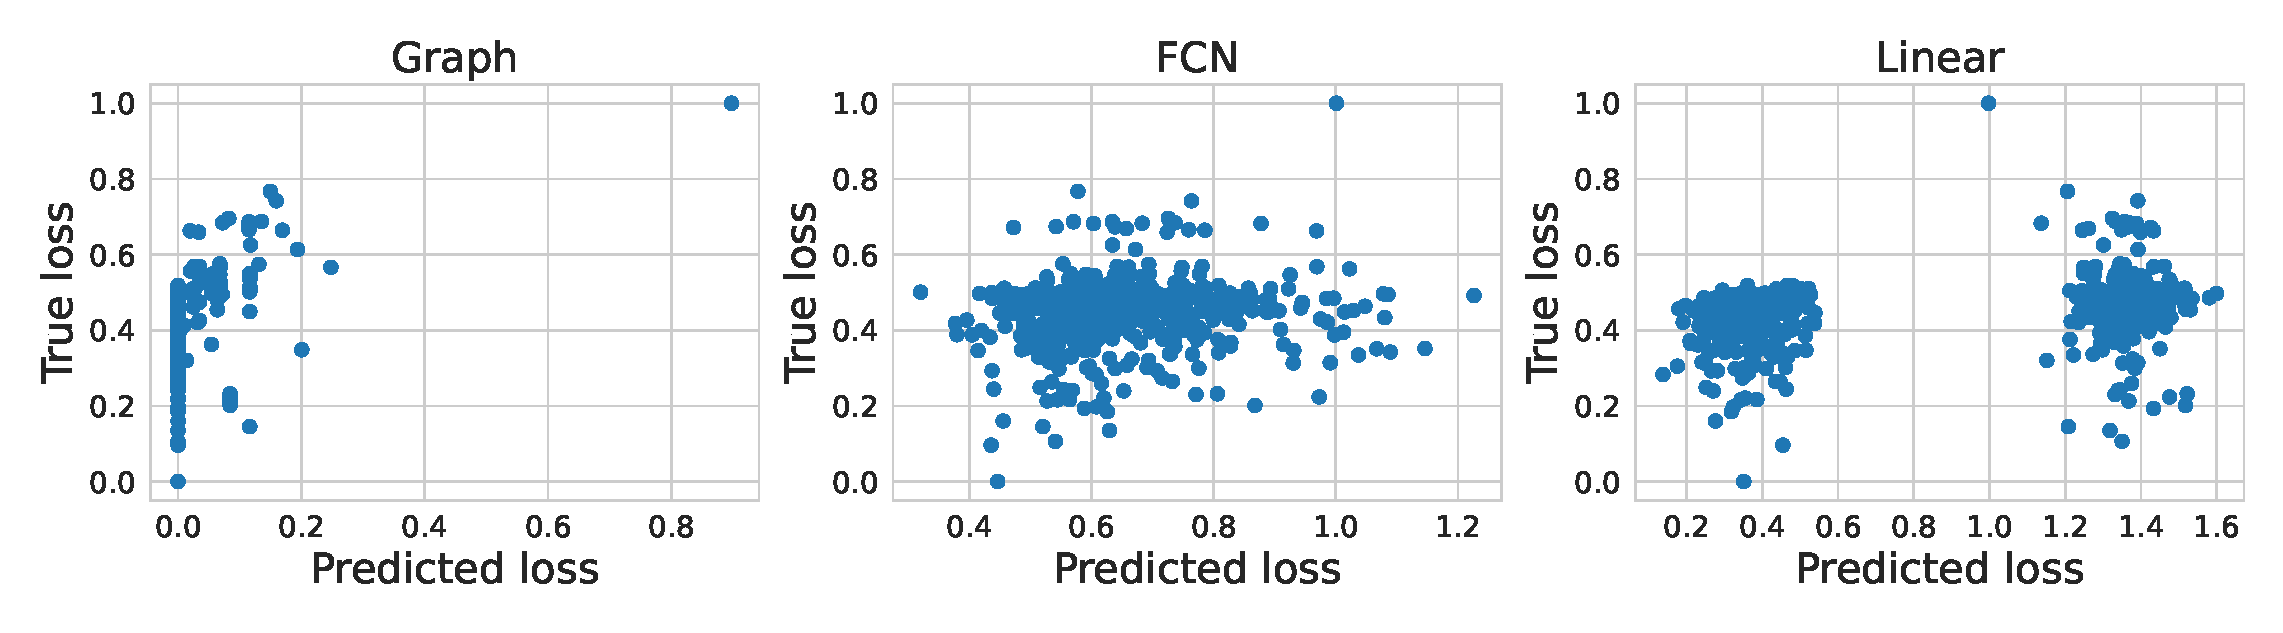
\includegraphics[width=\textwidth]{figs/graph_1_iter_14_experiment_6.eps}
\centering

\includegraphics[width=0.7\textwidth]{figs/graph_2_iter_14_experiment_6.eps}
\caption{Scatter plot of true and predicted error values for the baseline comparison. The parameter \texttt{n\_iterations} is set to 14.}
\label{graph_iter_14}
\end{figure}

\begin{figure}[H]
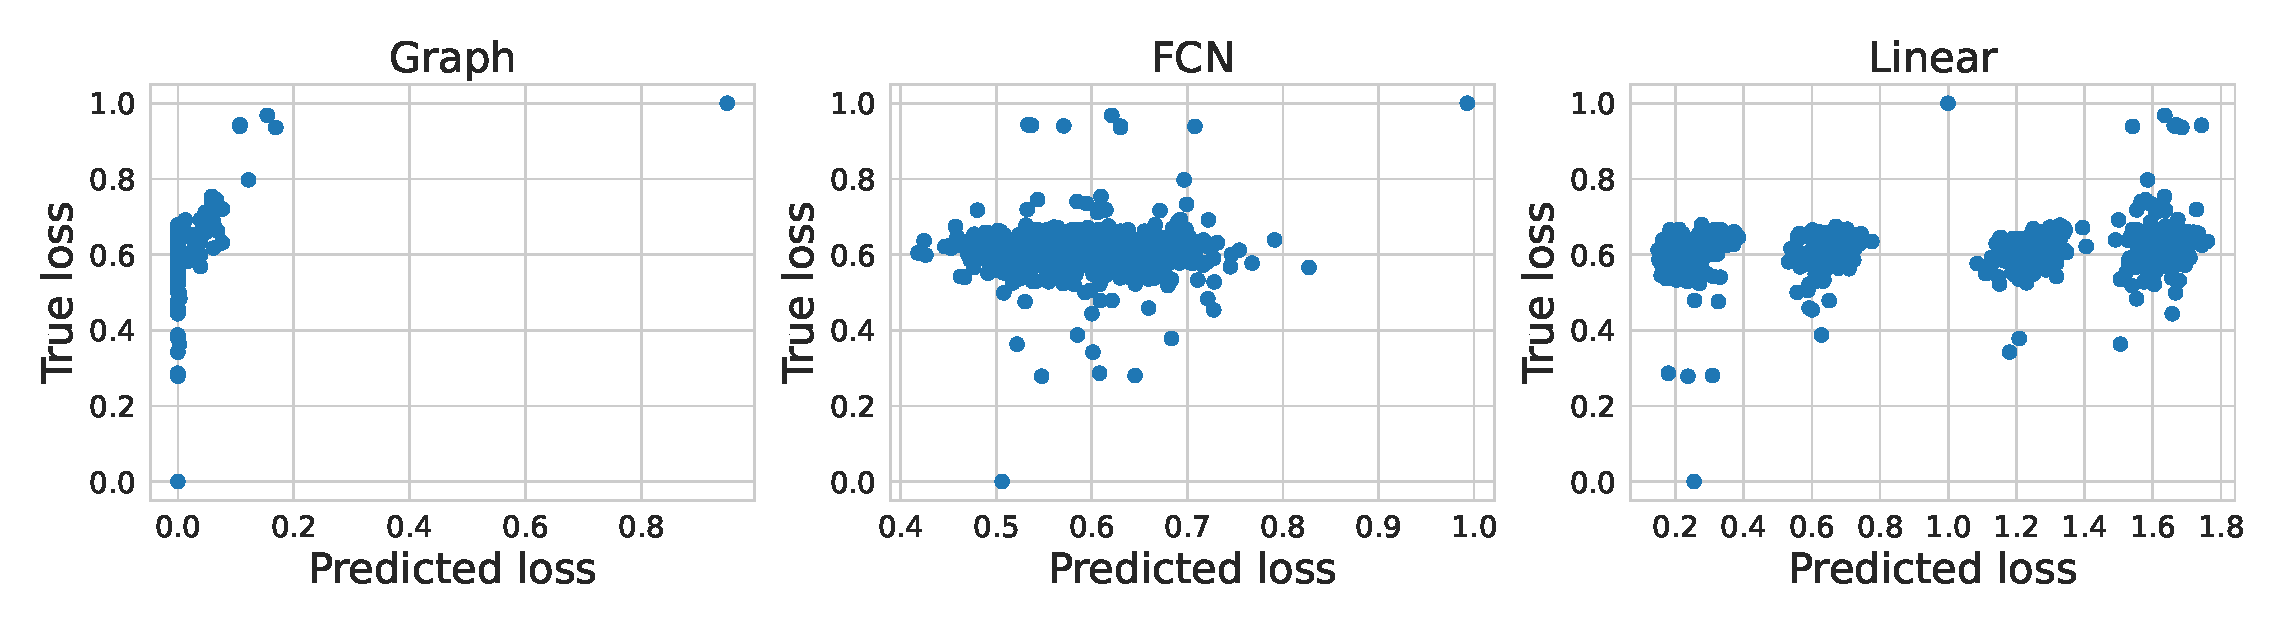
\includegraphics[width=\textwidth]{figs/graph_1_iter_30_experiment_6.eps}
\centering
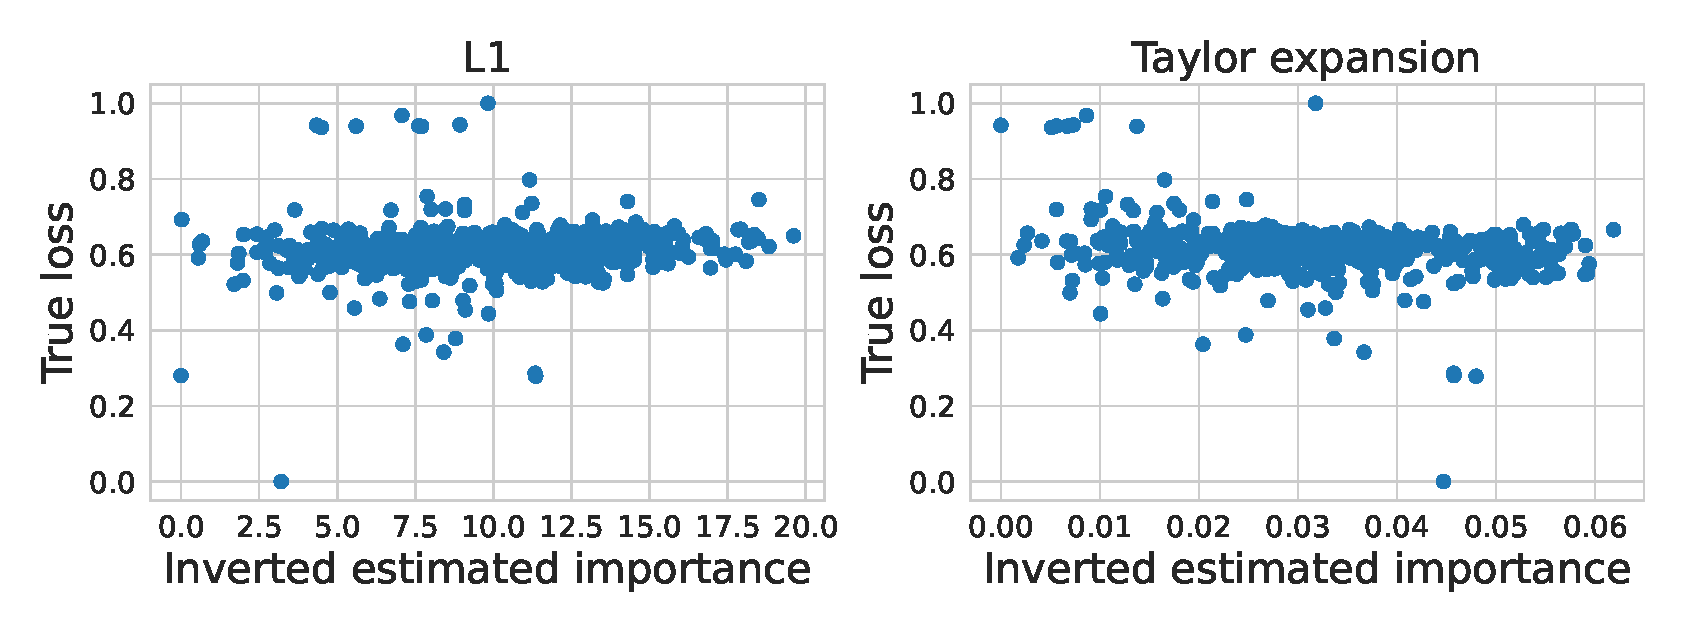
\includegraphics[width=0.7\textwidth]{figs/graph_2_iter_30_experiment_6.eps}
\caption{Scatter plot of true and predicted error values for the baseline comparison. The parameter \texttt{n\_iterations} is set to 30.}
\label{graph_iter_30}
\end{figure}

Additionally, scatter plots (Figs.~\ref{graph_iter_2}--\ref{graph_iter_30}) illustrate the relationship between true and predicted error values. 
In all considered cases, the surrogate graph model exhibits a stronger dependence between true and predicted errors than the baseline models. 
These visualizations are consistent with the correlation metrics reported above.

We compute the overlap between the top-$k$\% of models ranked according to the true loss and the top-$k$\% of models ranked according to the surrogate prediction. The resulting overlap ratio is used as a measure of prediction accuracy. To improve statistical stability, the experiment is repeated 10 times and the results are averaged. The results are presented in Tables~\ref{results_top5} and~\ref{results_top10}.

\begin{table}[H]
\caption{The overlap between the top-$5$\% of models ranked according to the true loss and the models ranked according to the surrogate prediction.}
\label{results_top5}
\centering
\begin{tabular}{|r|c|c|c|c|}
\hline
\bfseries Model & 10--15 edges & 20--40 edges & 50--100 edges & more than 100 edges \\
\hline
Graph  & \textbf{62.0\%} & \textbf{64.5\%} & \textbf{69.3\%} & \textbf{58.3\%} \\
FCN & 2\% & 15.2\% & 5.2\% & 6.8\% \\
Linear & 18.8\% & 9.6\% & 27.2\% & 15.2\% \\
L1 & 0.0\% & 1.6\% & 6.8\% & 6.8\% \\
Taylor expansion & 8.0\% & 10.8\% & 29.6\% & 24.4\% \\
\hline
\end{tabular}
\end{table}

\begin{table}[H]
\caption{The overlap between the top-$10$\% of models ranked according to the true loss and the models ranked according to the surrogate prediction.}
\label{results_top10}
\centering
\begin{tabular}{|r|c|c|c|c|}
\hline
\bfseries Model & 10--15 edges & 20--40 edges & 50--100 edges & more than 100 edges \\
\hline
Graph  & \textbf{55.3\%} & \textbf{54.8\%} & \textbf{67.4\%} & \textbf{66.9\%} \\
FCN & 7.4\% & 16.6\% & 12.4\% & 11.4\% \\
Linear & 22.6\% & 15.0\% & 28.6\% & 25.8\% \\
L1 & 2.0\% & 4.0\% & 12.0\% & 10.4\% \\
Taylor expansion & 12.6\% & 16.8\% & 30.0\% & 29.6\% \\
\hline
\end{tabular}
\end{table}

The plots in the (Fig.~\ref{final_plot}) indicate that, as the number of edges in the graph model increases, the proposed method achieves higher performance.

\begin{figure}[H]
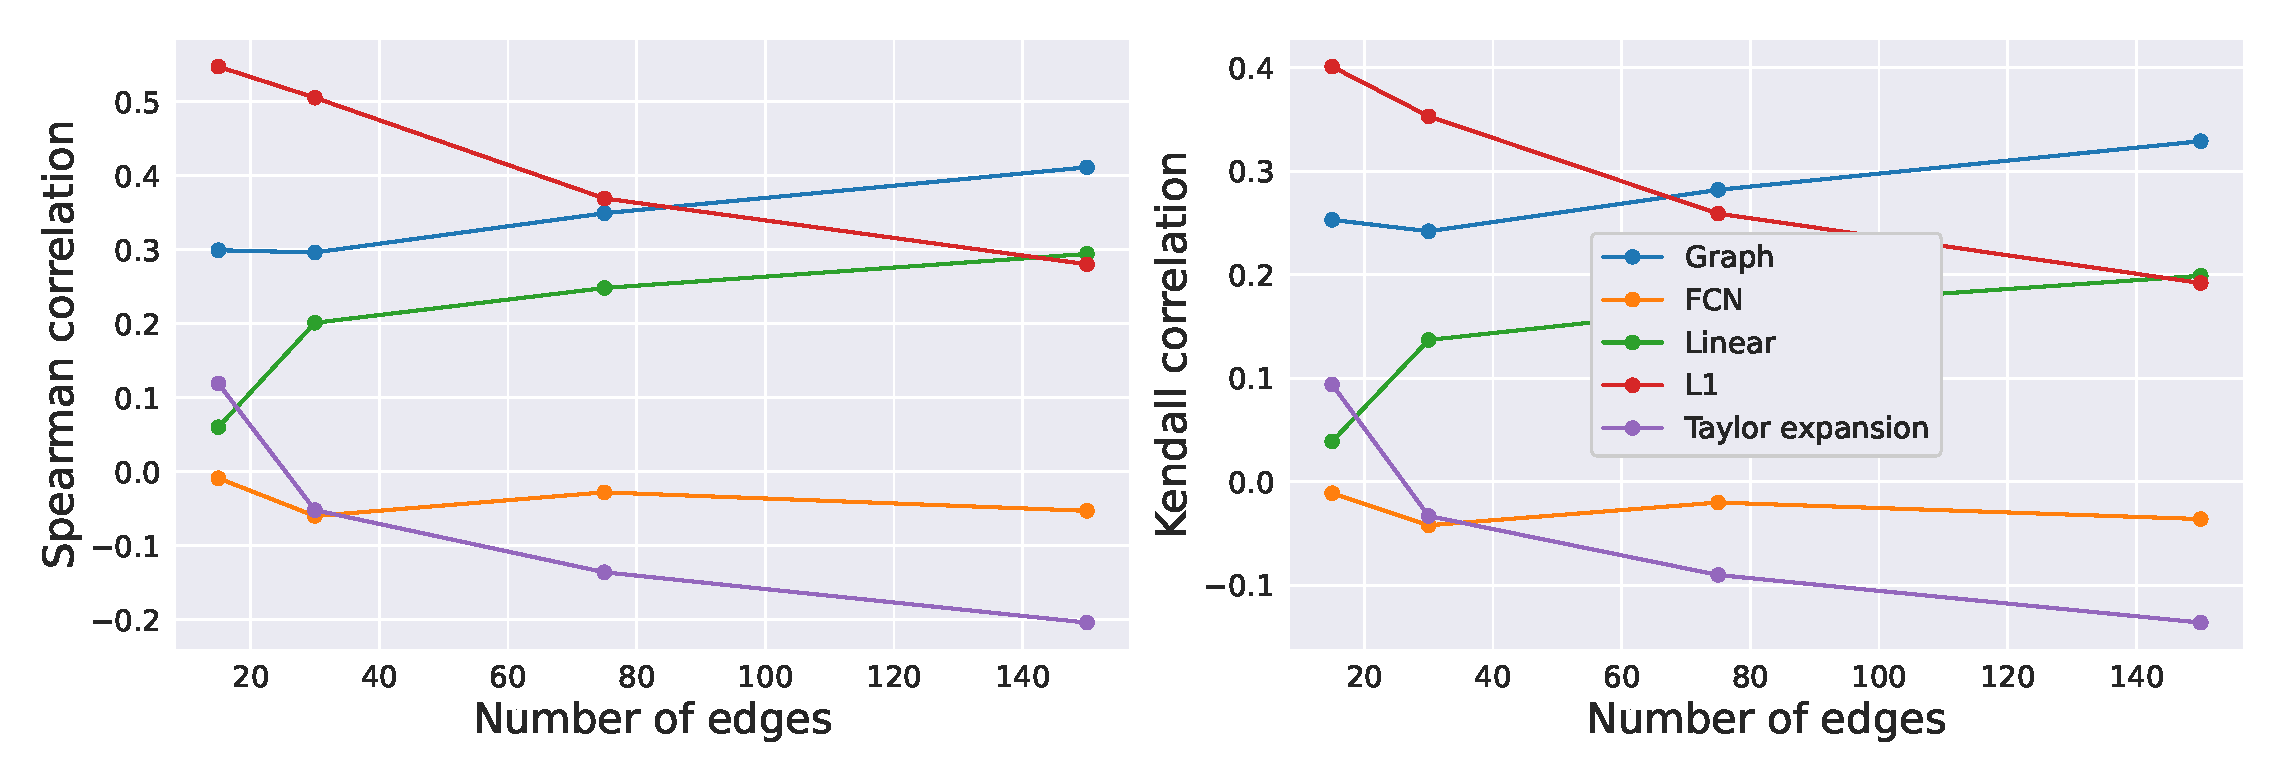
\includegraphics[width=\textwidth]{figs/final_plot.eps}
\caption{The plot shows the dependence of correlation coefficients on the number of edges.}
\label{final_plot}
\end{figure}